\chapter{Descripción del proyecto}
En este capítulo se describe cómo funciona el motor en esencia, es decir, sin entrar en la implementación del mismo. Esta idea general no depende del lenguaje de programación.

Hay un apartado que describe al motor y sus capacidades, y otro apartado que muestra el diseño actual de la aplicación y expone otras ideas que se pueden llevar a cabo.

\section{Qué es un motor de videojuegos (Descripción)}

El programa que se ha desarrollado es un motor que funciona como \textbf{intérprete de videojuegos}. Permite a un usuario cualquiera reproducir un videojuego definido en un formato predefinido. Este formato permite abstraer de toda la capa programática a un diseñador.

Aunque lo parezca, y quizás en una futura compilación sea capaz de hacerlo, no es una aplicación que permita crear un videojuego, sino que es capaz de reproducir videojuegos creados por un usuario.

El proyecto también se le puede definir como un motor de videojuegos:
\begin{quote}
	\small Un motor de videojuego es un término que hace referencia a una serie de librerías de programación que permiten el diseño, la creación y la representación de un videojuego. \cite{Alberto_Carrasco}
\end{quote}

En este caso, el proyecto no es una serie de librerías sino que es directamente una aplicación. De esta manera, se puede abstraer a un creador del videojuego de la programación directa de un juego.

\subsection{Qué tipo de videojuegos se pueden crear}
El interprete está orientado a reproducir juegos en los que el jugador tiene que escapar de una mazmorra. Para ello, el jugador debe reunir objetos como llaves para abrir puertas, esquivar trampas, resolver rompecabezas, luchar contra monstruos, usar pociones y llegar a una habitación final.
Algunos ejemplos de juegos parecidos a los que está orientado el motor son ''Dragones y Mazmorras'' o los libros de ''elige tu propia aventura''.

Aunque el motor esté desarrollado con una fuerte influencia por este tipo de juegos, no está limitado a ellos, cualquier creador pueda ir más allá de este concepto o incluso cambiarlo radicalmente usando las herramientas genéricas de las que dispone el motor. El límite lo pone la imaginación del usuario.

\subsection{Dónde se podrá usar el motor}
De momento sólo está disponible para dispositivos que soporten el sistema operativo iOS, es decir, solo para dispositivos portables de Apple, como un iPhone o un iPad.
Tampoco hay planes actuales de mover el motor a otra plataforma, pero es posible implementar el motor en otros sistemas y lenguajes de programación.

Con todas estas dudas resueltas ya solo queda mostrar las funciones de las que dispone el motor.

\subsection{Qué es capaz de hacer el motor}

El proyecto anterior se considera un punto de partida para muchos conceptos que se querían llevar a cabo para el nuevo motor. Por ello, se escogieron ciertas funcionalidades comunes que permitieran representar al videojuego original, separandolas en pequeñas piezas: mostrar un diálogo, iniciar un combate...
De esta manera nacen los \textbf{eventos}.

El juego original también contaba con una serie de jugadores con los que podía interactuar el usuario, salas en las que se desarrollaba la historia, un sistema de movimiento en forma de cuadrícula... Todos estos aspectos se han traducido al motor de manera que sean lo más fieles posibles al juego original.

A continuación, se describen por partes las funcionalidades que tiene el motor. De momento no se entra en las especificaciones propias de la implementación, pero aparecerá en la sección \ref{engineGuideSection}.

\subsection{Eventos}

Un evento representa una acción atómica que puede realizar el motor. Estas acciones se consideran básicas en el ámbito de una aventura, como escoger una opción o mostrar un diálogo; aunque requieran de más trabajo a la hora de programarlas.

Los eventos están pensados para unirse entre ellos, de manera que se puedan mezclar entre sí varias acciones básicas para formar una cadena de eventos. Por ello, cualquiera de ellos son intercambiables, intercalables y no pueden tener dependencias entre sí.
Además, siempre se ejecutan de forma lineal, siguiendo un orden predefinido por el creador del juego.

El centro de toda la potencia del motor reside en los eventos, ya que son un mecanismo genérico y preciso de ejecutar acciones en el juego. El motor está encargado de leer cada uno de estos eventos y ejecutar una acción según el contenido del mismo.
Otra funcionalidad clave del motor es que nunca sabe el estado en el que se encuentra la cadena de eventos, se conforma con guardar el evento que esté ejecutando en el momento, ejecutarlo y pasar al siguiente.

\begin{figure}[h]
	\caption{Cadena de eventos}
	\centering
	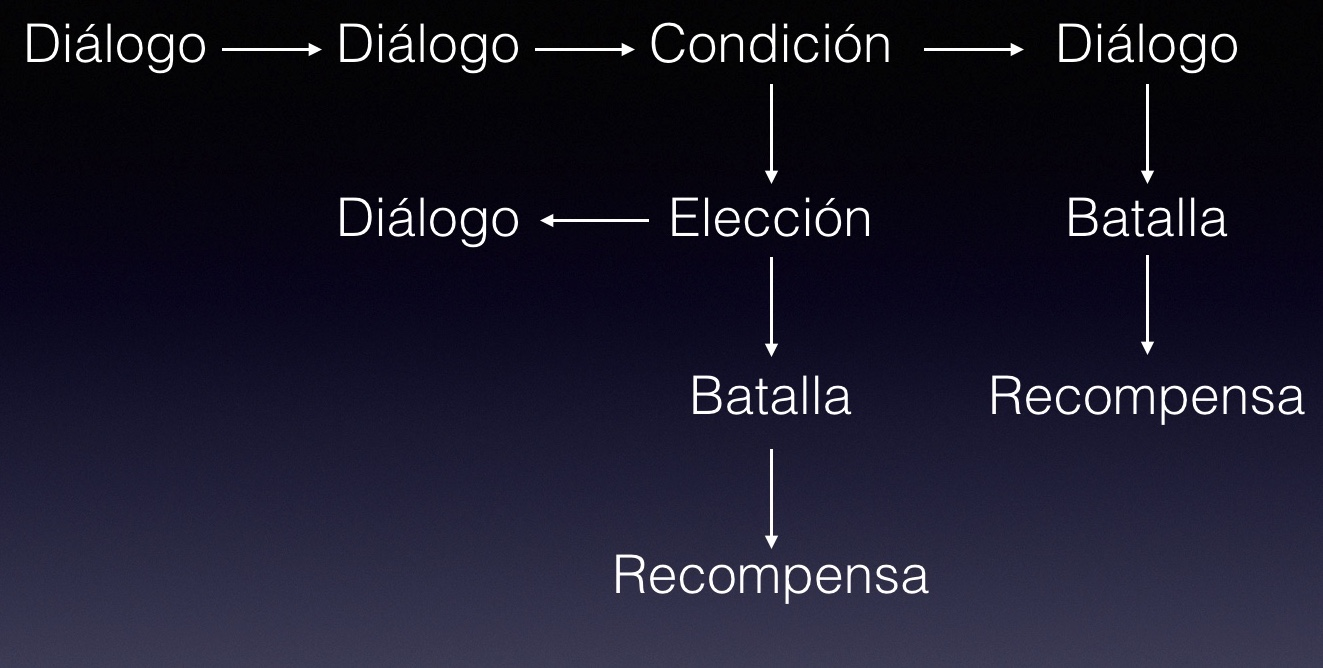
\includegraphics[width=0.75\textwidth]{include/eventsChainExample.jpg}
	
	La idea detrás de los eventos es muy sencilla: al interactuar el usuario con una parte de la aplicación activa una cadena. El evento principal tiene una referencia a otro evento, al que le da paso cuando termina el original. Este encadenamiento sigue hasta que uno de los eventos no tenga ninguna referencia a un evento siguiente, permitiendo que la cadena termine.
\end{figure}

Ahora vamos a definir los tipos de eventos que existen, las acciones que conllevan dentro del motor y sus posibles usos. Respecto a diseño que toman, se describirá más adelante en la sección de diseño \ref{designSection}. 

\subsubsection{Diálogo}
Evento que muestra un mensaje dicho por un personaje en el videojuego. La mayor traba del proyecto original era que los diálogos correspondían con la mayor parte del código fuente, por lo que este evento permite quitar mucha lógica duplicada en el código.

Su uso más frecuente es para mostrar conversaciones entre personajes, aunque también se puede usar para escribir los pensamientos del protagonista, describir una sala o un personaje, plantear un problema...

\subsubsection{Condición}
Evento que verifica una condición sobre el estado actual del juego. Este evento es transparente para el usuario, ya que se ejecutará un evento u otro siguiente dependiendo de si la condición es cierta o no. Las condiciones son las que se describen en la sección \ref{conditionsSubsection}.

Este evento se suele usar cuando se quiere evaluar el estado del juego y tomar acciones en consecuencia. Por ejemplo, diálogos dependientes del compañero, cofres que no se abren si no dispones de una llave...

\subsubsection{Elección}
Evento que permite al jugador escoger entre una serie de opciones. Dependiendo de la opción escogida, se ejecutará un evento u otro. Además, las opciones pueden incluir una condición para que se muestren, como las descritas en la sección \ref{conditionsSubsection}.

Algunos ejemplos en los que aparece este evento son cuando hay que resolver un acertijo y se muestran varias respuestas, o cuando un personaje te ofrece posibles formas de pago para un trueque.

\subsubsection{Batalla}
Evento que inicia una nueva batalla con la información de un enemigo al que enfrentarse.
Hasta que no termine la batalla no se pasará al siguiente evento de la cadena.

Al terminar la batalla se ejecutará un evento según si el jugador ha ganado o ha perdido.

\subsubsection{Recompensa}
Evento que agrega objetos al inventario del jugador. En ningún caso agregará objetos que no existan en el videojuego.

Se suele usar para recompensar a un jugador por haber ganado una batalla o por haber abierto un cofre.

\subsection{Habitaciones}
La idea original para el desarrollo del juego es un laberinto. Un laberinto se puede representar como una serie de pasillos delgados y oscuros por los que el protagonista debe orientarse, o como una serie de habitaciones interconectadas entre sí.
Esta última opción permite al jugador orientarse por cada partida, obtener mayor detalle sobre los eventos, recordar lugares memorables y ayudar a estructurar el laberinto para el usuario. 

Una habitación es el sitio donde ocurren todos los eventos que se pueden encontrar en el juego. Es en estos lugares donde el jugador va a tener mayor libertad de movimientos porque es el lugar donde se ejecutan cadenas de eventos, puede ir hacia otras habitaciones o donde puede guardar la partida y cambiar ciertos ajustes.

Está representada con una imagen principal que describe a la habitación junto con un título y una descripción, y una serie de acciones que puede realizar el jugador dentro de ella.

\subsection{Personajes}
Durante la aventura el protagonista puede interactuar con múltiples personajes: compañeros, enemigos y NPCs, las siglas de \textit{''non playable character''}. \cite{npcGeekno} Además, el jugador también cuenta como un personaje aparte.

Todos los personajes cuentan con un nombre y una imagen que los representa, y los compañeros y enemigos añaden una serie de características.
Las posibles estadísticas que puede tener un personaje son:

\begin{itemize}
	\item \textbf{Puntos de vida actuales}: representan la vida restante del personaje. Si los puntos de vida actuales del protagonista llegan a 0, entonces el juego termina.
	\item \textbf{Puntos de vida totales}: representan la vida máxima que tiene un personaje.
	\item \textbf{Puntos de ataque}: representan los puntos de vida actuales que puede quitar un personaje con un ataque.
	\item \textbf{Puntos de defensa}: representan los puntos de vida actuales que el personaje elimina de un ataque al recibirlo.
	\item \textbf{Puntos de agilidad}: representan la velocidad de un personaje. En un combate, si un personaje supera por un factor multiplicativo la agilidad del contrario, entonces el personaje puede atacar múltiples veces en un mismo turno. 
	\item \textbf{Estado alterado}: representa un cambio en el estado normal del personaje y pueden reportar beneficios o perjuicios al mismo. Los estados soportados por el motor son veneno, ceguera y parálisis.
	\item \textbf{Arma}: un personaje puede tener un arma consigo para atacar. Estas armas aumentarán el estado base de ataque, añadirán un porcentaje de acierto del ataque y un estado alterado a provocar.
\end{itemize}

Respecto a las tres últimas estadísticas, se explican con más detalle en el apartado de batalla de la sección de diseño \ref{battleDesignSubsection}.

Los personajes por lo tanto son piezas esenciales de la acción durante el juego por distintas razones:

\begin{itemize}
	\item Los diálogos siempre son enunciados por alguien, que debe ser un personaje. Un diálogo no se puede ejecutar si no existe un personaje que lo enuncie.
	\item El protagonista y su compañero tienen una serie de características que son cruciales para la evaluación de condiciones, como los indicadores de habitaciones visitadas.
	\item En una batalla, siempre lucha un personaje enemigo contra el protagonista y sus compañeros.
\end{itemize}

Además, usar personajes permite que los jugadores puedan adentrarse en la aventura con mayor facilidad e incluso identificarse con ellos.

\subsection{Condiciones} \label{conditionsSubsection}
El motor tiene varios puntos donde se necesita ejecutar condiciones para resolver ciertas acciones. Estas condiciones están sujetas a varios factores como las estadísticas del protagonista, valor de las variables internas, etc.

Existen varios tipos de evaluaciones:
\begin{itemize}
	\item Compañero: si el protagonista tiene un compañero que coincide con el nombre definido, entonces la condición se evalúa a verdadera. En otro caso, la condición es falsa.
	\item Objeto: si el protagonista tiene un objeto en su inventario que coincide con el objeto del evento, entonces la condición es cierta. En otro caso, no se cumple la condición. Es importante puntualizar que si la condición es cierta, entonces el objeto del inventario desaparece o se consume.
	\item Estado de habitación: dependiendo si el protagonista ha visitado una habitación específica o no, la condición se evalúa a cierto o falso. Hay una condición que sirve para saber si se ha visitado una habitación y otra para si no la ha visitado.
	\item Relación de variables: si la relación entre dos variables se cumple, entonces la condición es cierta. En otro caso, la condición es falsa. La relación de variables se describe mejor en la sección \ref{variablesSection}.
\end{itemize}

\subsection{Variables personalizadas} \label{variablesSection}

Esta es una nueva funcionalidad del motor que no se encontraba en la original.

Las variables personalizadas es una capacidad del juego que permite almacenar información dinámica de la partida, sin estar limitados por la propia capacidad del motor. Estas permiten a un diseñador de juegos controlar ciertos aspectos internos del juego como puede ser la activación de un evento o de ciertas elecciones.

Estas variables se pueden usar para guardar la información del estado de ejecución de un evento, almacenar la cantidad de tesoros que ha encontrado el jugador durante su partida...

De esta manera, la capacidad de formular condiciones aumenta sobremanera, ya que no dependen de las que puedan estar definidas en el motor. Es más, el diseñador del juego puede emular cualquier condición por defecto si usa las variables correctamente.

Las variables siempre tienen un id que las identifica, el dato que guarda y el tipo de ese dato. Una variable siempre se crea definiendo estos tres campos.
El motor soporta de momento los tipos entero, que representa números enteros; booleano, que representa valores de verdad, como verdadero y falso; y cadena de texto, que son un literal de texto.

Debido a que estas variables son dinámicas, el motor permite no solo sustituir el valor o crear nuevas variables, sino que también permite operaciones entre variables o más datos estáticos.

Las operaciones estarán formadas por dos variables y la operación que realizan entre ellos. Las operaciones soportadas por el motor dependen del tipo de dato que guarde la variable, y nunca podrán operarse dos variables con distintos tipos de datos. El resultado de la operación siempre se guarda en la primera variable con la que se opera.

\begin{itemize}
	\item Las variables \textbf{enteras} soportan las operaciones sustituir, suma, resta, multiplicación, división entera y módulo/resto.
	\item Las variables \textbf{booleanas} soportan las operaciones sustituir, conjunción, disyunción y negación.
	\item Las variables que son \textbf{cadenas de texto} permiten sustituir el texto o concatenarlo.
\end{itemize}

A continuación se describe lo que realiza cada operación:

\begin{itemize}
	\item \textbf{Sustituir}: modifica el valor anterior de la variable con uno nuevo.
	\item \textbf{Disyunción}: ejecuta la operación disyunción booleana sobre la primera y la segunda variable.
	\item \textbf{Conjunción}: ejecuta la operación conjunción booleana sobre la primera y la segunda variable.
	\item \textbf{Negación}: ejecuta la operación negación booleana sobre la segunda variable.
	\item \textbf{Suma}: suma el valor de la primera variable con el de la segunda.
	\item \textbf{Resta}: resta el valor de la primera variable con el de la segunda.
	\item \textbf{Multiplicación}: multiplica el valor de la primera variable por el de la segunda.
	\item \textbf{División entera}: realiza la división entera del valor de la primera variable con el de la segunda.
	\item \textbf{Resto}: halla el resto de la división entera entre el valor de la primera variable y el de la segunda.
	\item \textbf{Sustituir}: concatena el texto de la primera variable con el de la segunda.
\end{itemize}

Con todas estas operaciones se pueden modificar el contenido de las variables, mediante una segunda variable u otro dato estático.

El uso principal de las variables, cuando ya tienen un valor, es el evaluar su valor comparándolo con otra variable o un dato estático. Para ello, el motor permite realizar operaciones de comparación, y al igual que las operaciones de modificación solo funcionan si los dos tipos de las variables a comparar son iguales. En este caso los operadores son compatibles para todos los tipos de variables, aunque su funcionalidad cambie.

Los operadores disponibles son igual, distinto, mayor, mayor o igual, menor y menor o igual. A continuación se describe la comparación que se realiza dependiendo del operador. La condición es cierta:

\begin{itemize}
	\item Operadores enteros:
	\begin{itemize}
		\item \textbf{Igual}: si los dos enteros son iguales.
		\item \textbf{Distinto}: si los dos enteros son distintos.
		\item \textbf{Mayor}: si el primer entero es mayor que el segundo.
		\item \textbf{Mayor o igual}: si el primer entero es mayor que el segundo o si son iguales.
		\item \textbf{Menor}: si el primer entero es menor que el segundo.
		\item \textbf{Menor o igual}: si el primer entero es menor que el segundo o si son iguales.
	\end{itemize}
	\item Operadores booleanos:
	\begin{itemize}
		\item \textbf{Igual}: si los dos valores son iguales.
		\item \textbf{Distinto}: si los dos valores son distintos.
		\item \textbf{Mayor}: si el primer valor es verdadero y el segundo es falso.
		\item \textbf{Mayor o igual}: si el primero es verdadero o si los dos son falsos.
		\item \textbf{Menor}: si el primero es falso y el segundo es verdadero.
		\item \textbf{Menor o igual}: si el primero es falso o si los dos son verdaderos.
	\end{itemize}
	\item Operadores de cadenas de texto:
	\begin{itemize}
		\item \textbf{Igual}: si las dos cadenas son iguales.
		\item \textbf{Distinto}: si las dos cadenas son distintas.
		\item \textbf{Mayor}: si la primera cadena se sitúa posteriormente a la otra según el orden lexicográfico.
		\item \textbf{Mayor o igual}: si la primera cadena se sitúa posteriormente a la otra según el orden lexicográfico o si las cadenas son iguales.
		\item \textbf{Menor}: si la primera cadena se sitúa anteriormente a la otra según el orden lexicográfico.
		\item \textbf{Menor o igual}: si la primera cadena se sitúa anteriormente a la otra según el orden lexicográfico o si las cadenas son iguales.
	\end{itemize}
\end{itemize}
 
\section{Qué esperar del sistema (Diseño)} \label{designSection}

\subsection{Batalla} \label{battleDesignSubsection}

\section{Cómo se ve el motor en funcionamiento}

\section{Guía para usar el sistema} \label{engineGuideSection}

Antes de comenzar, todos los eventos tienen una serie de características comunes entre ellos:

\begin{itemize}
	\item Identificador: todos los eventos cuentan con un id, y este debe ser único. No se asegura que dos eventos con identificadores idénticos funcionen a la vez.
	\item Siguiente paso: indica el identificador del próximo evento a ejecutarse...
	akbhdfdkjalskshbebbjdkjbajbkRELLENAR
\end{itemize}

Para crear un videojuego disponemos de x archivos.
Describir cada uno y explicar en qué se traduce en el juego



\chapter{Desarrollo de la aplicación}

\section{Una manera de llevarlo a cabo (Arquitectura)}

\section{Desarrollando en dispositivos móviles (Implementación)}